\documentclass{article}
\usepackage{fullpage}
\usepackage{amsmath}
\usepackage{amsfonts}
\usepackage{graphicx}

\title{User Manual for \texttt{DS\_BN\_v2.exe} (version 2)}
\author{Shawn Eastwood}
\date{}

\begin{document}

\maketitle

\section{About}

\texttt{DS\_BN\_v2.exe} is a software tool that facilitates probabilistic inference using Markov networks, Bayesian networks, and their Dempster-Shafer equivalents \cite{[Eastwood2015]}. The current build (version 2.0) runs on Windows 7, service pack 1.


\section{Introduction}

\texttt{DS\_BN\_v2.exe} on startup requests an unsigned integer $i$ that is used to identify the input files from which variable and factor data is loaded. Once $i$ is provided, $4$ files are accessed by \texttt{DS\_BN\_v2.exe}:
\begin{description}
\item[\texttt{$i$\_Variables\_file.txt}] contains information about the variables to be used in the simulation.
\item[\texttt{$i$\_Factors\_file.txt}] contains information about the tabular classical Markov network factors to be used in the simulation.
\item[\texttt{$i$\_DS\_Factors\_file.txt}] contains information about the tabular Dempster-Shafer factors to be used in the simulation.
\item[\texttt{$i$\_Instructions\_file.txt}] contains a series of instructions on the operations to be preformed on the provided factors.
\end{description}  
Output from the program is printed to the console, as well as written to the file \texttt{$i$\_Output\_file.txt}

The following sections will list the data format required for each of the $4$ input files. In each .txt file, the amount and type of whitespace between the tokens is irrelevant. 



\section{\texttt{$i$\_Variables\_file.txt}}

In laying out the expected format for \texttt{$i$\_Variables\_file.txt}, the following notation will be used:
\begin{itemize} 
\item $N$ is an integer that denotes the total number of variables to be used in the simulation. Theoretically, $0 \leq N \leq 2^{31} - 1$ as $N$ is stored as a signed integer. 
\item $s(j)$ is a string that denotes the name of the $j^\text{th}$ variable. $s(j)$ cannot have any whitespace. 
\item $n(j)$ is the domain size of the $j^\text{th}$ variable. Theoretically, $0 \leq n(j) \leq 2^{31} - 1$ as $n(j)$ is stored as a signed integer.
\end{itemize}

This information is stored in \texttt{$i$\_Variables\_file.txt} via the following format:
\begin{verbatim}
N

s(1) n(1)
s(2) n(2)
...
s(N) n(N)
\end{verbatim}



\section{\texttt{$i$\_Factors\_file.txt}}

In laying out the expected format for \texttt{$i$\_Factors\_file.txt}, the following notation will be used:
\begin{itemize}
\item Let $N$ is an integer that denotes the total number of tabular Markov network factors to be used in the simulation. Theoretically, $0 \leq N \leq 2^{31} - 1$ as $N$ is stored as a signed integer. 
\item $n(j)$ denotes the number of variables that the $j^\text{th}$ factor covers. Again $0 \leq n(j) \leq 2^{31} - 1$. It should be noted that a factor can have 0 variables. 
\item $s(j,k)$ denotes the name of the $k^\text{th}$ variable from the $j^\text{th}$ factor. 
\item $M(j)$ is the total number of possible assignments to the variables in the $j^\text{th}$ factor. It must be the case that the total number of assignments to the variables in the $j^\text{th}$ factor be $\leq 2^{31} - 1$
\item In a tabular factor, the factor's values will be listed in a linear array indexed by the variables. The array is ordered so that the latter variables cycle the fastest. $f(j,k)$ denotes the $k^\text{th}$ entry in the linear array. It should be noted that a factor that covers no variables has exactly one variable assignment, and therefore 1 value entry.
\end{itemize}

The factor information is stored in \texttt{$i$\_Factors\_file.txt} via the following format:
\begin{verbatim}
N

n(1)
s(1,1) s(1,2) ... s(1,n(1))
f(1,1) f(1,2) f(1,3) ... f(1,M(1))

n(2)
s(2,1) s(2,2) ... s(2,n(2))
f(2,1) f(2,2) f(2,3) ... f(2,M(2))

...

n(N)
s(N,1) s(N,2) ... s(N,n(N))
f(N,1) f(N,2) f(N,3) ... f(N,M(N))
\end{verbatim} 



\section{\texttt{$i$\_DS\_Factors\_file.txt}}

In laying out the expected format for \texttt{$i$\_DS\_Factors\_file.txt}, the following notation will be used:
\begin{itemize}
\item $N$ is an integer that denotes that total number of tabular Dempster-Shafer factors to be used in the simulation. Theoretically, $0 \leq N \leq 2^{31} - 1$ as $N$ is stored as a signed integer. 
\item $n(j)$ denotes the number of variables that the $j^\text{th}$ factor covers. Again $0 \leq n(j) \leq 2^{31} - 1$. It should be noted that a factor can have 0 variables. 
\item $s(j,k)$ denotes the name of the $k^\text{th}$ variable from the $j^\text{th}$ factor. 
\item $M(j)$ is the total number of possible assignments to the variables in the $j^\text{th}$ factor. It must be the case that the total number of assignments to the variables in the $j^\text{th}$ factor be $\leq 2^{31} - 1$
\item $L(j)$ is the number of focal elements associated with the $j^\text{th}$ factor. $1 \leq L(j) \leq 2^{31} - 1$. There can be 0 focal elements, which denotes the ``zero Dempster-Shafer factor".
\item $f(j,k)$ is the weight of the $k^\text{th}$ focal element of the $j^\text{th}$ factor.
\item A focal element of the $j^\text{th}$ factor is denoted using a linear array indexed by the variables of the $j^\text{th}$ factor. The array is ordered so that the latter variables cycle the fastest. Each entry of the array is a true/false value that indicates if the variable assignment that indexes the array location belongs to the focal element. $b(j,k,l) \in \{0,1\}$ denotes the $l^\text{th}$ array entry of the $k^\text{th}$ focal element of the $j^\text{th}$ factor. 
\end{itemize}

The DS factor information is stored in \texttt{$i$\_DS\_Factors\_file.txt} via the following format:
\begin{verbatim}
N

n(1)
s(1,1) s(1,2) ... s(1,n(1))
L(1)
f(1,1) b(1,1,1) b(1,1,2) b(1,1,3) ... b(1,1,M(1))
f(1,2) b(1,2,1) b(1,2,2) b(1,2,3) ... b(1,2,M(1))
...
f(1,L(1)) b(1,L(1),1) b(1,L(1),2) b(1,L(1),3) ... b(1,L(1),M(1))

n(2)
s(2,1) s(2,2) ... s(2,n(2))
L(2)
f(2,1) b(2,1,1) b(2,1,2) b(1,1,3) ... b(2,1,M(2))
f(2,2) b(2,2,1) b(2,2,2) b(1,2,3) ... b(2,2,M(2))
...
f(2,L(2)) b(2,L(2),1) b(2,L(2),2) b(2,L(2),3) ... b(2,L(2),M(2))

...

n(N)
s(N,1) s(N,2) ... s(N,n(N))
L(N)
f(N,1) b(N,1,1) b(N,1,2) b(N,1,3) ... b(N,1,M(N))
f(N,2) b(N,2,1) b(N,2,2) b(N,2,3) ... b(N,2,M(2))
...
f(N,L(N)) b(N,L(N),1) b(N,L(N),2) b(N,L(N),3) ... b(N,L(N),M(N))
\end{verbatim}



\section{\texttt{$i$\_Instructions\_file.txt}}

The instructions file communicates to \texttt{Uncertainty\_Classes.exe} what is to be done with uploaded variable and factor data. Instructions have the following format:
\begin{verbatim}
%factor_type #command arg1 arg2 ... argN
\end{verbatim} 
Like with the previous files, the amount and type of whitespace between the tokens is irrelevant. 

\texttt{\%factor\_type} is replaced with either \texttt{\%Tabular\_Factor} or \texttt{\%Tabular\_DS\_Factor} depending of the type of factors that the command is referring to.

Variables are referenced by their string name; the $j^\text{th}$ Markov network factor is referenced by the token: \texttt{Fj}; and the $j^\text{th}$ Dempster-Shafer factor is referenced by the same token: \texttt{Fj}. A Markov network factor and a Dempster-Shafer factor can be referenced by the same token since the token \texttt{\%factor\_type} at the start of each command indicates the type of factor(s) involved. When a new factor is created, it must be referenced by a token. New tokens do not need to be declared. When a factor is written to an existing token, the factor aliased by that token is overwritten.

The commands are:
\begin{description}
\item[\texttt{\#assign arg1 arg2}] ~~~ Copies the factor referenced by \texttt{arg2} into \texttt{arg1}. 
\item[\texttt{\#multiply dest N arg1 arg2 ... argN}] ~~~ Multiplies together the \texttt{N} factors \texttt{arg1}, \texttt{arg2}, \dots, \texttt{argN} and writes the result into \texttt{dest}. If \(N = 0\), a factor over 0 variables is returned that consists of a single ``1" in the case of Markov network factors; and a single all encompassing focal element with a weight of 1 in the case of Dempster-Shafer factors. 
\item[\texttt{\#marginalize fact N var1 var2 ... varN}] ~~~ Marginalizes factor \texttt{fact} with respect to the \texttt{N} variables \texttt{var1}, \texttt{var2}, \dots, \texttt{varN}. Factor \texttt{fact} must contain all \texttt{N} variables, and a variable cannot be repeated in the list.
\item[\texttt{\#condition fact N var1 val1 var2 val2 .... varN valN}] ~~~ Conditions factor \texttt{fact} by fixing the value of variable \texttt{var1} to \texttt{val1}; \texttt{var2} to \texttt{val2}; and so on. If \(m\) is the domain size of variable \(x\), then the value assigned to \(x\) is a number from $\{0, 1, \dots, m-1\}$. Unlike \texttt{\#marginalize}, factor \texttt{fact} does not need to contain all \texttt{N} variables, but a variable cannot be repeated in the list.
\item[\texttt{\#normalize fact}] ~~~ Normalizes the weights in factor \texttt{fact} so that they sum to 1.
\item[\texttt{\#print fact}] ~~~ Prints the factor \texttt{fact} to both the console and the output file \texttt{$i$\_Output\_file.txt}
\item[\texttt{\#balloon fact N var1 val1 var2 val2 ... varN valN}] ~~~ \textbf{(This command only applies to tabular Dempster-Shafer factors.)} Dempster-Shafer factor \texttt{fact} is extended to cover variables \texttt{var1}, \texttt{var2}, \dots, \texttt{varN} via the ``ballooning extension" \cite{[Eastwood2015]}.  The existing factor exists at the assignment \texttt{var1 = val1}; \texttt{var2 = val2}; \dots; \texttt{varN = valN}. None of \texttt{var1}, \texttt{var2}, \dots, \texttt{varN} can be already present in \texttt{fact}, nor can a variable be repeated.
\end{description}

Moreover, comments can be introduced into the instructions file by beginning a comment with the token \texttt{/*} and ending the comment with the token \texttt{*/}. Both \texttt{/*} and \texttt{*/} must be padded on both sides by whitespace.




\section{Examples}\label{sec:Examples}

\subsection{Example 1}\label{sec:Example_1}

Consider the Markov network in figure \ref{fig:Belief_network_1}.

\begin{figure}[!h]
\begin{center}
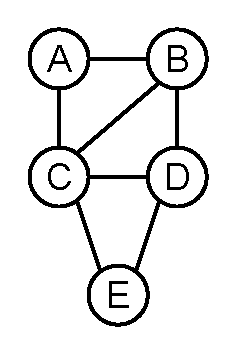
\includegraphics{fig/Belief_network_1}
\caption{The Markov network used in the example in section \ref{sec:Example_1}.}
\label{fig:Belief_network_1}
\end{center}
\end{figure}

Imagine that we wish to conduct numerical inference using the network in figure \ref{fig:Belief_network_1}. The files will be indexed with \(i = 1\). The variables are described in the file ``\texttt{1\_Variables\_file.txt}":
\begin{verbatim}
5

A 2
B 3
C 2
D 3
E 2
\end{verbatim}

Assume that there are 4 Markov network factors, covering the variable sets \(\{A\}\); \(\{A, B, C\}\); \(\{B, C, D\}\); and \(\{C, D, E\}\). These factors are described in the file ``\texttt{1\_Factors\_file.txt}":
\begin{verbatim}
4

1
A
1.0  2.0

3
A B C
1.0  2.0  3.0  4.0  5.0  6.0  
0.0  0.0  0.0  0.0  0.0  0.0

3
B C D
1.0  2.0  3.0  4.0  5.0  6.0
0.0  0.0  0.0  0.0  0.0  0.0
1.0  1.0  1.0  1.0  1.0  1.0

3
C D E
1.0  0.0  0.0  1.0  1.0  0.0  
0.0  0.0  0.0  0.0  0.0  0.0
\end{verbatim}

I will also give 4 Dempster-Shafer factors that cover the same sets of variables as the Markov network factors. While these factors cover the same sets of variables as the Markov network factors, their focal elements and weights will have no meaningful relation to the Markov network factors. These factors are described in the file ``\texttt{1\_DS\_Factors\_file.txt"}:
\begin{verbatim}
4

1
A
1
2.0 1 1

3
A B C
1
3.0 1 1 1 1 1 1
    0 0 0 0 0 0

3
B C D
2
1.0 1 1 1 1 1 1
    0 0 0 0 0 0
    0 0 0 0 0 0
2.0 0 0 0 0 0 0
    0 0 0 0 0 0
    1 1 1 1 1 1

3
C D E
3
1.0 1 0 0 0 0 0
    0 0 0 0 0 0
1.0 0 0 0 1 0 0
    0 0 0 0 0 0
1.0 0 0 0 0 1 0
    0 0 0 0 0 0
\end{verbatim}

 
As an example of inference involving Markov network, I will apply the evidence \(B = 0\) and \(D = 0\) to each of the factors (note that \texttt{\#condition} ignores variables that are not in the factor). I will then multiply together all of the factors and marginalize with respect to variables \(A\) and \(C\). I will normalize the quantities in the resulting factor over \(E\) and print the result. This is implemented for both Markov network factors and Dempster-Shafer factors in the file ``\texttt{1\_Instructions\_file.txt}":
\begin{verbatim}
/* Copy and condition each Tabular_Factor: */

%Tabular_Factor #assign F1_temp F1
%Tabular_Factor #condition F1_temp 2 B 0 D 0

%Tabular_Factor #assign F2_temp F2
%Tabular_Factor #condition F2_temp 2 B 0 D 0

%Tabular_Factor #assign F3_temp F3
%Tabular_Factor #condition F3_temp 2 B 0 D 0

%Tabular_Factor #assign F4_temp F4
%Tabular_Factor #condition F4_temp 2 B 0 D 0

/* Form and marginalize the product: */

%Tabular_Factor #multiply Fprod 4 F1_temp F2_temp F3_temp F4_temp
%Tabular_Factor #marginalize Fprod 2 A C
%Tabular_Factor #normalize Fprod 
%Tabular_Factor #print Fprod



/* Repeat for Tabular_DS_Factor: */

%Tabular_DS_Factor #assign F1_temp F1
%Tabular_DS_Factor #condition F1_temp 2 B 0 D 0

%Tabular_DS_Factor #assign F2_temp F2
%Tabular_DS_Factor #condition F2_temp 2 B 0 D 0

%Tabular_DS_Factor #assign F3_temp F3
%Tabular_DS_Factor #condition F3_temp 2 B 0 D 0

%Tabular_DS_Factor #assign F4_temp F4
%Tabular_DS_Factor #condition F4_temp 2 B 0 D 0

%Tabular_DS_Factor #multiply Fprod 4 F1_temp F2_temp F3_temp F4_temp
%Tabular_DS_Factor #marginalize Fprod 2 A C
%Tabular_DS_Factor #normalize Fprod 
%Tabular_DS_Factor #print Fprod
\end{verbatim}

The output that is printed to the console and to the file ``\texttt{1\_Output\_file.txt}" is:
\begin{verbatim}
1
E 
1 0 


1
E 
1
1 1 0 
\end{verbatim}



\subsection{Example 2}\label{sec:Example_2}

This next example will use the Dempster-Shafer Bayesian network example from \cite[sections 8.6, 8.7, 8.8]{[EastwoodCIDS2015]}. This example demonstrates use of the ballooning extension. The example is given below:

The following variables form the belief network in Fig. \ref{fig:Belief_network_3}.

Variable \(S\) denotes the scenario currently taking place; 
\(\text{Val}(S) = \{s_1, s_2, s_3, s_4, s_5\}\) where
\begin{itemize}
\item \(s_1\) denotes a normal situation where the traveler holds an e-passport belonging to his/herself. 
\item \(s_2\) denotes a situation where the traveler has lost their e-passport.
\item \(s_3\) denotes a situation where the traveler is attempting to use an e-passport that they have stolen.
\end{itemize}

 Variable \(L\) denotes whether or not the e-passport has been reported as lost;
$\text{Val}(L) = \{l_1, l_2\}$ where
 \(l_1\) indicates that the passport has been reported as lost, and
 \(l_2\) indicates that the passport has not been reported as lost.

 Variable \(W\) denotes whether or not the e-passport is on a watchlist for being fraudulently obtained or not;
$\text{Val}(W) = \{w_1, w_2\}$ where
\(w_1\) indicates that the e-passport is on a watchlist, and
 \(w_2\) indicates that the e-passport is not on a watchlist.

\begin{figure}[!hbt]
\begin{center}
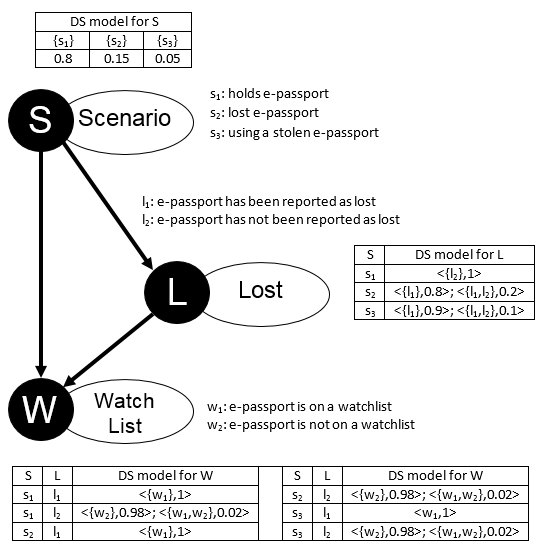
\includegraphics[natwidth=572,natheight=530,width=0.8\textwidth]{fig/Belief_network_3.png}
\end{center}
 \caption{The DST Bayesian network that is used for the example in section  \ref{sec:Example_2}. Each DS model is denoted using a list of focal element, weight pairs: $\langle B, m(B)\rangle$}
\label{fig:Belief_network_3}
\end{figure}

Next, a ``conditional Dempster-Shafer table'' is assigned to each node as indicated in Fig. \ref{fig:Belief_network_3}.  

%The DST model associated with variable \(S\) is \(\langle \{s_1\}, 0.8\rangle\); \(\langle \{s_2\}, 0.15\rangle\); \(\langle \{s_3\}, 0.05\rangle\). A DST model is expressed as a series of $\langle$ focal element, weight $\rangle$ pairs: \(\langle B, m(B) \rangle\). 
%This DST model indicates that with probability \(0.8\) we know that the traveler holds their own e-passport; with probability \(0.15\) we know that the traveler does not currently possess an e-passport; and with probability \(0.05\) we know that the traveler is engaged in illegal activity. The CDSTs associated with variables \(L\) and \(W\) are listed in Table \ref{tab:CDSTs}.
%
%\begin{table}[h!]
%\begin{center}
%\begin{small}
%\begin{tabular}{cc}
%\parbox{0.5\textwidth}{
%\begin{tabular}{|c|c|}
%\hline
%\(S\) & DS models for \(L\) \\
%\hline
%\(s_1\) & \(\langle \{l_2\}, 1\rangle\) \\
%\(s_2\) & \(\langle \{l_1\}, 0.8\rangle\); \(\langle \{l_1, l_2\}, 0.2\rangle\) \\
%\(s_3\) & \(\langle \{l_1\}, 0.9\rangle\); \(\langle \{l_1, l_2\}, 0.1\rangle\) \\
%\hline
%\end{tabular}} & 
%\parbox{0.5\textwidth}{
%\begin{tabular}{|c|c|c|}
%\hline
%\(S\) & \(L\) & DS models for \(W\) \\
%\hline
%\(s_1\) & \(l_1\) & \(\langle \{w_1\}, 1\rangle\) \\
%\(s_1\) & \(l_2\) & \(\langle \{w_1, w_2\}, 0.02\rangle\); \(\langle \{w_2\}, 0.98\rangle\) \\
%\(s_2\) & \(l_1\) & \(\langle \{w_1\}, 1\rangle\) \\
%\(s_2\) & \(l_2\) & \(\langle \{w_1, w_2\}, 0.02\rangle\); \(\langle \{w_2\}, 0.98\rangle\) \\
%\(s_3\) & \(l_1\) & \(\langle \{w_1\}, 1\rangle\) \\
%\(s_3\) & \(l_2\) & \(\langle \{w_1, w_2\}, 0.02\rangle\); \(\langle \{w_2\}, 0.98\rangle\) \\
%\hline
%\end{tabular}}
%\end{tabular}
%\end{small}
%\end{center}
%\caption{CDSTs for \(L\) and \(W\).}
%\label{tab:CDSTs}
%\end{table}

\begin{sloppypar}
On the website ``\texttt{<http://www.ucalgary.ca/btlab/Software>}", files ``\texttt{3\_Variables\_file.txt}" and ``\texttt{3\_DS\_Factors\_file.txt}" encode the variables and Dempster-Shafer factors listed above and in Fig. \ref{fig:Belief_network_3}. The file ``\texttt{3\_Factors\_file.txt}" contains a single ``0". There are a total of 10 Dempster-Shafer factors: 1 for \(S\); 3 for \(L\); and 6 for \(W\). Note that each Dempster-Shafer factor carries no information about the parents of the corresponding variable, or the row's placement in the conditional Dempster-Shafer table.  
\end{sloppypar}



\subsubsection{Inference using the DST based belief network}

First, we derive the total DST model that is described by the above DS-BN. This is done using ballooning extensions and the following commands from the file ``\texttt{3\_Instructions\_file.txt}":

\begin{verbatim}
%Tabular_DS_Factor #assign D_S F1

/* Multiply together all Dempster-Shafer factors associated with L */
%Tabular_DS_Factor #assign D_L_0 F2
%Tabular_DS_Factor #balloon D_L_0 1 S 0
%Tabular_DS_Factor #assign D_L_1 F3
%Tabular_DS_Factor #balloon D_L_1 1 S 1
%Tabular_DS_Factor #assign D_L_2 F4
%Tabular_DS_Factor #balloon D_L_2 1 S 2
%Tabular_DS_Factor #multiply D_L 3 D_L_0 D_L_1 D_L_2
%Tabular_DS_Factor #print D_L

/* Multiply together all Dempster-Shafer factors associated with W */
%Tabular_DS_Factor #assign D_W_00 F5
%Tabular_DS_Factor #balloon D_W_00 2 S 0 L 0
%Tabular_DS_Factor #assign D_W_01 F6
%Tabular_DS_Factor #balloon D_W_01 2 S 0 L 1
%Tabular_DS_Factor #assign D_W_10 F7
%Tabular_DS_Factor #balloon D_W_10 2 S 1 L 0
%Tabular_DS_Factor #assign D_W_11 F8
%Tabular_DS_Factor #balloon D_W_11 2 S 1 L 1
%Tabular_DS_Factor #assign D_W_20 F9
%Tabular_DS_Factor #balloon D_W_20 2 S 2 L 0
%Tabular_DS_Factor #assign D_W_21 F10
%Tabular_DS_Factor #balloon D_W_21 2 S 2 L 1
%Tabular_DS_Factor #multiply D_W 6 D_W_00 D_W_01 D_W_10 D_W_11 D_W_20 D_W_21
%Tabular_DS_Factor #print D_W

/* Multiply together the S and L factors */
%Tabular_DS_Factor #multiply D_SL 2 D_S D_L
%Tabular_DS_Factor #print D_SL

/* Multiply together the S, L and W factors */
%Tabular_DS_Factor #multiply D_SLW 2 D_SL D_W
%Tabular_DS_Factor #print D_SLW
\end{verbatim}

The total DST model is built by first deriving a DSF from each row of each CDST. There is one DSF associated with \(S\), 3 DSFs associated with \(L\), and 6 DSFs associated with \(W\). 
The one DSF associated with \(S\) will be denoted by \(F_S\).

Below, the calculations performed by \texttt{DS\_BN\_v2.exe} are performed by hand below:

%\subsubsection
{Step I:}
The product of the 3 DST factors associated with \(L\),  denoted by \(D_L\), is shown below. Let \(sl\)  denote an arbitrary assignment to variables \(S\) and \(L\) where \(s\) is the assignment to \(S\) and \(l\) is the assignment to \(L\).

\begin{center}
\begin{small}
\begin{tabular}{|c|c||c|c|}
\hline
Focal Element & Weight& Focal Element & Weight\\
\hline
\(\{s_1l_2, s_2l_1, s_3l_1\}\) & 0.72& \(\{s_1l_2, s_2l_1, s_2l_2, s_3l_1\}\) & 0.18\\
\(\{s_1l_2, s_2l_1, s_3l_1, s_3l_2\}\) & 0.08 &\(\{s_1l_2, s_2l_1, s_2l_2, s_3l_1, s_3l_2\}\) & 0.02\\
\hline
\end{tabular}
\end{small}
\end{center}

%\subsubsection*
{Step II:}
The product of the 6 DST factors associated with \(W\), denoted by \(D_W\), is shown below. To simplify notation, \(slw\)  denotes an arbitrary assignment to variables \(S\), \(L\), and \(W\) where \(s\) is the assignment to \(S\), \(l\) is the assignment to \(L\), and \(w\) is the assignment to \(W\).
\begin{center}
\begin{small}
\begin{tabular}{|c|c|c|c|c|}
\hline 
Focal Element & Weight & ~~~~ & Focal Element & Weight \\
\hline
\(\{s_1l_1w_1, s_1l_2w_1, s_1l_2w_2, \dots\) & &                  & \(\{s_1l_1w_1, s_1l_2w_2, \dots\)  & \\
\(\dots, s_2l_1w_1, s_2l_2w_1, s_2l_2w_2, \dots\) & &          & \(\dots, s_2l_1w_1, s_2l_2w_1, s_2l_2w_2, \dots\) & \\
\(\dots s_3l_1w_1, s_3l_2w_1, s_3l_2w_2\}\) & 0.000008 &  & \(\dots s_3l_1w_1, s_3l_2w_1, s_3l_2w_2\}\) & 0.000392 
\\
\(\{s_1l_1w_1, s_1l_2w_1, s_1l_2w_2, \dots\) & &                 & \(\{s_1l_1w_1, s_1l_2w_2, \dots\) & \\
\(\dots s_2l_1w_1, s_2l_2w_1, s_2l_2w_2, \dots\) & &          & \(\dots s_2l_1w_1, s_2l_2w_1, s_2l_2w_2, \dots\) & \\
\(\dots s_3l_1w_1, s_3l_2w_2\}\) & 0.000392 &                     & \(\dots s_3l_1w_1, s_3l_2w_2\}\) & 0.019208 
\\
\(\{s_1l_1w_1, s_1l_2w_1, s_1l_2w_2, \dots\) & &                & \(\{s_1l_1w_1, s_1l_2w_2, \dots\) & \\
\(\dots s_2l_1w_1, s_2l_2w_2, \dots\) & &                             & \(\dots s_2l_1w_1, s_2l_2w_2, \dots\) & \\
\(\dots s_3l_1w_1, s_3l_2w_1, s_3l_2w_2\}\) & 0.000392 & & \(\dots s_3l_1w_1, s_3l_2w_1, s_3l_2w_2\}\) & 0.019208  
\\
\(\{s_1l_1w_1, s_1l_2w_1, s_1l_2w_2, \dots\) & &                & \(\{s_1l_1w_1, s_1l_2w_2, \dots\) & \\
\(\dots s_2l_1w_1, s_2l_2w_2, \dots\) & &                             & \(\dots s_2l_1w_1, s_2l_2w_2, \dots\) & \\
\(\dots s_3l_1w_1, s_3l_2w_2\}\) & 0.019208 &                    & \(\dots s_3l_1w_1, s_3l_2w_2\}\) & 0.941192 \\
\hline
\end{tabular}
\end{small}
\end{center}


%\subsubsection
{Step III:}
Let us compute the product: \(D_{S,L} = D_S \times D_L\). The result  is shown below:
\begin{center}
\begin{small}
\begin{tabular}{|c|c|}
\hline
Focal Element & Weight \\
\hline
\(\{s_1l_2\}\) & \(0.8 \cdot (0.72 + 0.08 + 0.18 + 0.02) = 0.8\) \\
\(\{s_2l_1\}\) & \(0.15 \cdot (0.72 + 0.08) = 0.12\) \\
\(\{s_2l_1, s_2l_2\}\) & \(0.15 \cdot (0.18 + 0.02) = 0.03\) \\
\(\{s_3l_1\}\) & \(0.05 \cdot (0.72 + 0.18) = 0.045\) \\
\(\{s_3l_1, s_3l_2\}\) & \(0.05 \cdot (0.08 + 0.02) = 0.005\) \\
\hline
\end{tabular}
\end{small}
\end{center}



%\subsubsection
{Step IV:}
Next, we compute the product: \(D_{S,L,W} = D_{S,L} \times D_W\), as shown below:
\begin{center}
\begin{small}
\begin{tabular}{|c|c|}
\hline
Focal Element & Weight \\
\hline
\(\{s_1l_2w_1, s_1l_2w_2\}\) & \(0.8 \cdot (0.000008 + 0.000392 + 0.000392 + 0.019208) = 0.016\) \\
\(\{s_1l_2w_2\}\) & \(0.8 \cdot (0.000392 + 0.019208 + 0.019208 + 0.941192) = 0.784\) \\
\(\{s_2l_1w_1\}\) & \(0.12 \cdot (0.000008 + 0.000392 + 0.000392 + 0.019208 + \dots\) \\
& \(\dots 0.000392 + 0.019208 + 0.019208 + 0.941192) = 0.12\) \\
\(\{s_2l_1w_1, s_2l_2w_1, s_2l_2w_2\}\) & \(0.03 \cdot (0.000008 + 0.000392 + 0.000392 + 0.019208) = 0.0006\) \\
\(\{s_2l_1w_1, s_2l_2w_2\}\) & \(0.03 \cdot (0.000392 + 0.019208 + 0.019208 + 0.941192) = 0.0294\) \\
\(\{s_3l_1w_1\}\) & \(0.045 \cdot (0.000008 + 0.000392 + 0.000392 + 0.019208 + \dots\) \\
& \(\dots 0.000392 + 0.019208 + 0.019208 + 0.941192) = 0.045\) \\
\(\{s_3l_1w_1, s_3l_2w_1, s_3l_2w_2\}\) & \(0.005 \cdot (0.000008 + 0.000392 + 0.000392 + 0.019208) = 0.0001\) \\
\(\{s_3l_1w_1, s_3l_2w_2\}\) & \(0.005 \cdot (0.000392 + 0.019208 + 0.019208 + 0.941192) = 0.0049\) \\
\hline
\end{tabular}
\end{small}
\end{center}


The above table simplifies to:
\begin{center}
\begin{small}
\begin{tabular}{|c|c||c|c|}
\hline
Focal Element & Weight &Focal Element & Weight \\
\hline
\(\{s_1l_2w_1, s_1l_2w_2\}\) & \(0.016\) &\(\{s_2l_1w_1, s_2l_2w_2\}\) & \(0.0294\) \\
\(\{s_1l_2w_2\}\) & \(0.784\) &\(\{s_3l_1w_1\}\) & \(0.045\)\\
\(\{s_2l_1w_1\}\) & \(0.12\) &\(\{s_3l_1w_1, s_3l_2w_1, s_3l_2w_2\}\) & \(0.0001\)\\
\(\{s_2l_1w_1, s_2l_2w_1, s_2l_2w_2\}\) & \(0.0006\) &\(\{s_3l_1w_1, s_3l_2w_2\}\) & \(0.0049\)\\
\hline
\end{tabular}
\end{small}
\end{center}
which is the total DST model for the DS-BN for this example.

Note that the commands from the file ``\texttt{3\_Instructions\_file.txt}" print \(D_L\), \(D_W\), \(D_{S,L}\), and \(D_{S,L,W}\). 

\subsubsection{Example of an inference problem: e-passport lost}

Let us consider the inference problem where the e-passport has been reported as being lost \(L = l_1\). We wish to compute the belief and plausibility that the e-passport is simply lost and not stolen \(S = s_2\).
To start, we derive the conditional DST model by applying the evidence \(L = l_1\) to the total DST model \(D_{S,L,W}\) computed previously. The variable \(W\) is then marginalized out. This process is captured by the instructions:
\begin{verbatim}
/* Condition and marginalize as per the inference example. */
%Tabular_DS_Factor #assign D1 D_SLW
%Tabular_DS_Factor #condition D1 1 L 0
%Tabular_DS_Factor #normalize D1
%Tabular_DS_Factor #print D1
%Tabular_DS_Factor #marginalize D1 1 W
%Tabular_DS_Factor #print D1
\end{verbatim}
Conditioning gives:
\begin{center}
\begin{small}
\begin{tabular}{|c|c|}
\hline
Focal Element & Weight \\
\hline
\(\{s_3w_1\}\) & \(\frac{1}{M}(0.12 + 0.0006 + 0.0294) = \frac{1}{0.15 + 0.05}0.15 = 0.75\) \\
\(\{s_4w_1\}\) & \(\frac{1}{M}(0.045 + 0.0001 + 0.0049) = \frac{1}{0.15 + 0.05}0.05 = 0.25\) \\
\hline
\end{tabular}
\end{small}
\end{center}
Marginalizing out variable \(W\) gives $\{s_3\}=0.75$ and $\{s_4\}=0.25$
We finally see that \(\text{Bel}(s_3|l_1) = \text{Pl}(s_3|l_1) = 0.75.\)

The output file can be found at: \texttt{<http://www.ucalgary.ca/btlab/Software>}. As can be seen all files for this example are indexed by \(i = 3\). 


\section*{Future Extensions}

In later versions of \texttt{DS\_BN.exe}, support for Dezert-Smarandache theory will be introduced.



\begin{thebibliography}{9}

\bibitem{[EastwoodCIDS2015]}
Eastwood, S. C.*, and S. N. Yanushkevich, Risk Assessment in Authentication Machines, \emph{Recent Advances in Computational Intelligence in Defense and Security}, 2015, 30 pages.

\bibitem{[Eastwood2015]}
Eastwood, S. C., and S. N. Yanushkevich, Graphical Dempster-Shafer Models of Uncertainty, submitted to \emph{Knowledge-Based Systems,} Elsevier (reference available upon request).

\end{thebibliography}

\end{document}


